\section{Foundations and Motivation}

\subsection{From ``Fail-Stop'' to ``Byzantine Fault''}
In the 1980s, fault tolerance research was heavily concentrated on \textit{fail-stop} faults, which occur when a node simply ceases to operate, typically due to a hardware crash. However, as systems grew more complex, these failures became just the tip of the iceberg. 

A node can fail due to software bugs or be compromised by malicious attackers. In these scenarios, the defective node does not shut down; it continues to communicate but can behave arbitrarily or transmit false information. This arbitrary behavior is known as a \textbf{Byzantine Fault}. Within a Byzantine environment, it is assumed that defective nodes actively conspire to corrupt the system state.

\subsection{The pBFT System Model}
The pBFT algorithm assumes a realistic and hostile system model:
\begin{itemize}
    \item \textbf{Asynchrony:} It operates in an asynchronous distributed system, such as the Internet, where messages can be delayed, lost, or delivered out of order.
    \item \textbf{Strong Adversary:} It posits an adversary capable of coordinating compromised nodes. pBFT relies heavily on cryptography (public-key signatures, MACs, cryptographic digests) to secure message integrity.
    \item \textbf{Safety without Synchrony:} It guarantees its safety property (contradictory operations will never be committed) regardless of network delays, relying only on weak synchrony for liveness.
\end{itemize}

\subsection{The $3f+1$ Rule}
To tolerate $f$ Byzantine failures, the minimum number of replicas required is $n = 3f+1$. This is because the protocol must be able to make progress using responses from $n - f$ replicas (since $f$ nodes could be dead or unresponsive). Within those received responses, $f$ nodes could be malicious liars. For the honest nodes' votes to strictly outvote the malicious ones, the following inequality must hold: $(n - f) - f > f \implies n > 3f$.

Another perspective to understand this rule is through quorum intersections. Committing an operation requires a quorum of $2f+1$ identical responses. If two distinct quorums of $2f+1$ intersect, their mathematical overlap will always contain at least $f+1$ replicas, inherently guaranteeing at least one honest node in the intersection.

\begin{figure}[H]
\centering
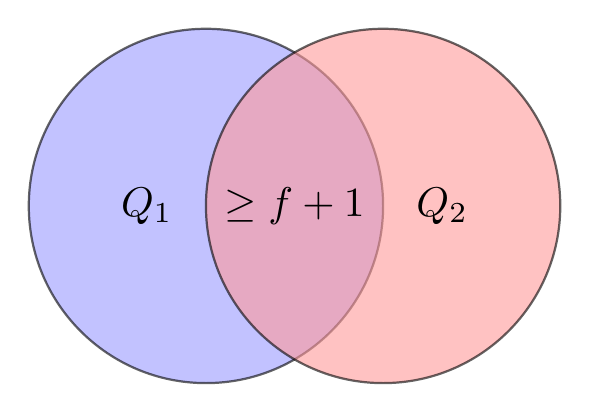
\begin{tikzpicture}[scale=1.5, every node/.style={transform shape}]
    \draw[fill=blue!40, opacity=0.6, draw=black, thick] (0,0) circle (1.5);
    \draw[fill=red!40, opacity=0.6, draw=black, thick] (1.5,0) circle (1.5);
    \node[text=black, font=\bfseries] at (-0.5,0) {$Q_1$};
    \node[text=black, font=\bfseries] at (2.0,0) {$Q_2$};
    \node[text=black, font=\bfseries] at (0.75,0) {$\ge f+1$};
\end{tikzpicture}
\caption{Quorum Intersection in pBFT}
\end{figure}